\chapter{Abordagem de desenvolvimento}

Este projeto terá diversas funcionalidades que se relacionam entre si, para organizar e sistematizar o processo de desenvolvimento foi usado uma adaptação do Scrum\footnote{https://www.scrum.org/} o Scrum Solo\footnote{https://engenhariasoftware.wordpress.com/2016/04/17/scrum-solo-2/}. O Scrum Solo é a combinação do framework Scrum Personal Software Process (PSP), onde:

\begin{citacao}
O Scrum é um framework ágil para gerenciamento de projetos que se destaca por sua abordagem enxuta (lean) de desenvolvimento. Por ser um modelo iterativo e incremental, o Scrum divide o projeto em vários sprints (ciclos curtos de desenvolvimento) consecutivos que ocorrerão de acordo com a prioridade do product owner (proprietário do produto). Cada período de sprint é definido, geralmente, entre duas e quatro semanas. Durante esse tempo, o scrum team (analista e programadores) se dedica ao máximo para ter um pequeno conjunto de funcionalidades codificadas e testadas. (ScrumSolo, 2017) O PSP é um processo de melhoria projetado para ajudar os desenvolvedores a controlar, administrar e aperfeiçoar sua competência para produzir software de qualidade. O propósito do PSP é ajudar o desenvolvedor a melhorar a sua forma de trabalho, entendendo sua própria performance e sabendo onde e como melhorá-la. A filosofia por trás do PSP é que a competência de uma organização para construir softwares de determinado tamanho e grau de complexidade decorre, em parte, da habilidade individual de seus engenheiros. O PSP se baseia no princípio do conhecimento, avaliação e melhorias contínuas do processo individual. \cite{ScrumSolo2017}
\end{citacao}

A Figura \ref{scrum} mostra como funciona os ciclos de iterações dentro do Framework Scrum Solo.

\begin{figure}[H]
\caption{\label{scrum} Funcionamento do Scrum solo}
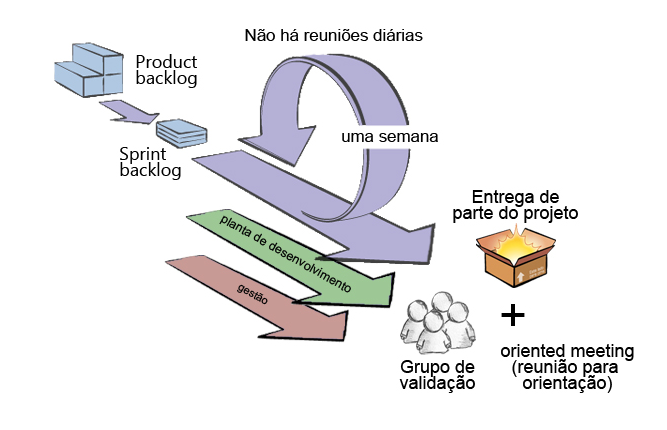
\includegraphics[scale=0.33]{img/scrum-solo.png}
\legend{Fonte: Website do Scrum Solo}
\end{figure}

As subseções a seguir apresentam a sequencia de etapas para facilitar o acompanhamento e a execução do projeto propostas pelo framework Scrum Solo.

\section{Levantamento de requisitos}
Esta é a primeira etapa do framework, aqui é feito a descrição dos principais pontos do software aplicados a solução do problema, para isso os seguintes artefatos são gerados:

\begin{itemize}
    \item[a)] Documento de escopo;
    \item[b)] Product Backlog;
    \item[c)] Protótipos de software.
\end{itemize}

A Figura \ref{sprints} mostra como estes artefatos estão relacionados com os atores nesta etapa.

\begin{figure}[H]
\caption{\label{sprints} Levantamento de requisitos}
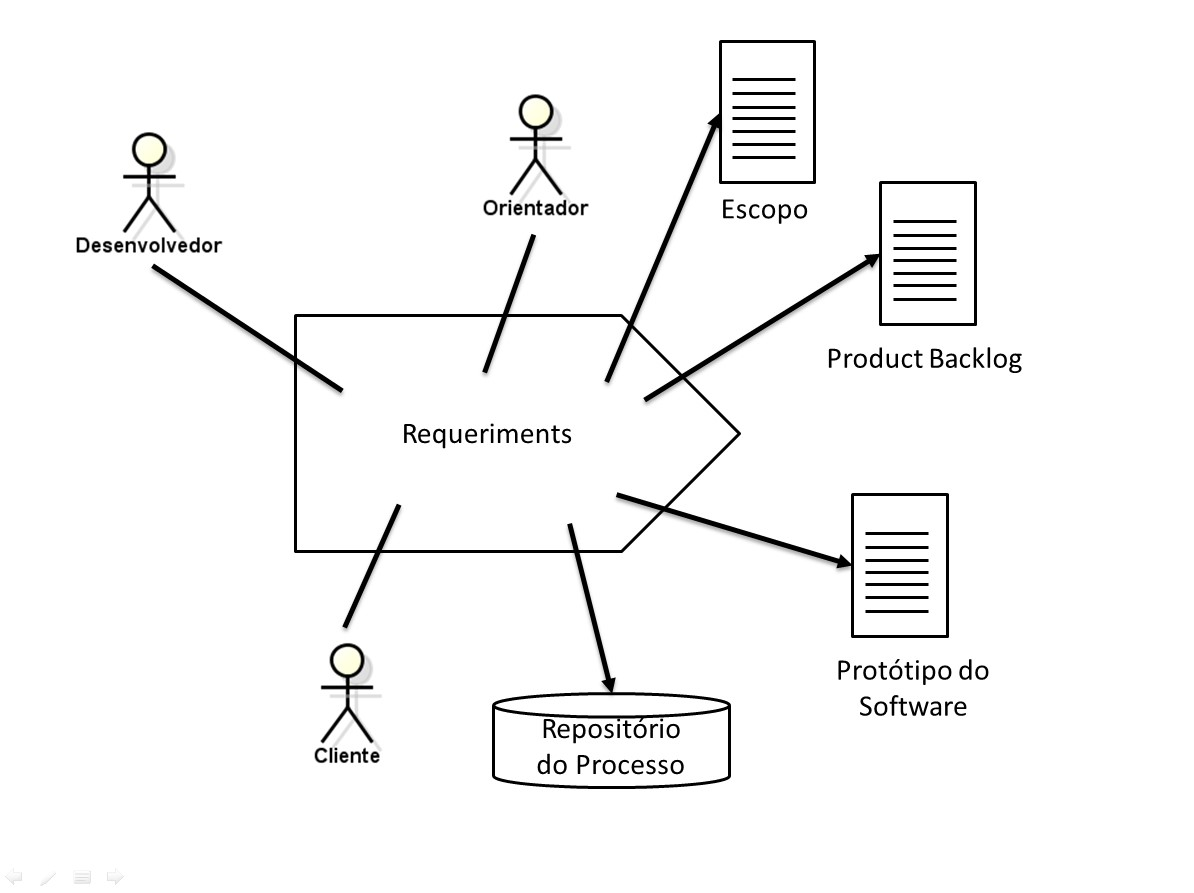
\includegraphics[scale=0.33]{img/levantamento-requisitos.jpg}
\legend{Fonte: Website do Scrum Solo}
\end{figure}

\section{Sprint}
Esta etapa, que pode ocorrer N vezes dentro de um projeto, movimenta os artefatos anteriores e faz a adição dos seguintes:

\begin{itemize}
    \item[a)] Sprint Backlog;
    \item[b)] Planta de desenvolvimento, este relatório;
    \item[c)] Ata de reunião, substituído por encontros regulares com o orientador e por análise deste relatório em documento de revisão;
    \item[d)] Produto parcial, com alguma funcionalidade pronta.
\end{itemize}

A Figura \ref{requisitos} mostra como fica o relacionamento entre os atores e os referidos artefatos.

\begin{figure}[H]
\caption{\label{requisitos} Manipulação de artefatos na Sprint}
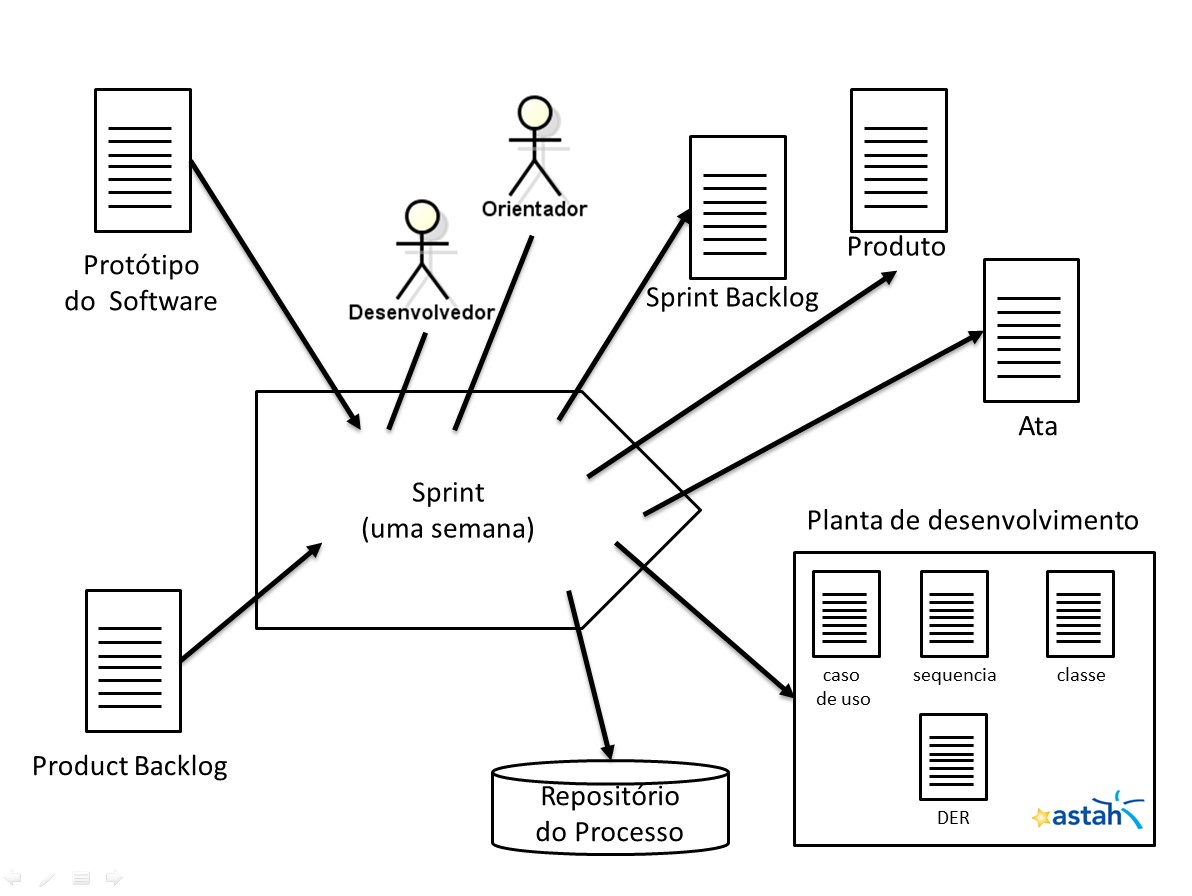
\includegraphics[scale=0.33]{img/sprints.jpg}
\legend{Fonte: Website do Scrum Solo}
\end{figure}

\section{Entrega}
Periodicamente é definido uma etapa de entrega, onde um conjunto de funcionalidades prontas e testadas é apresentado e entregue para o cliente, a Figura \ref{entrega} mostra como é o relacionamento dos atores com os artefatos nesta etapa.

\begin{figure}[H]
\caption{\label{entrega} Entrega de software}
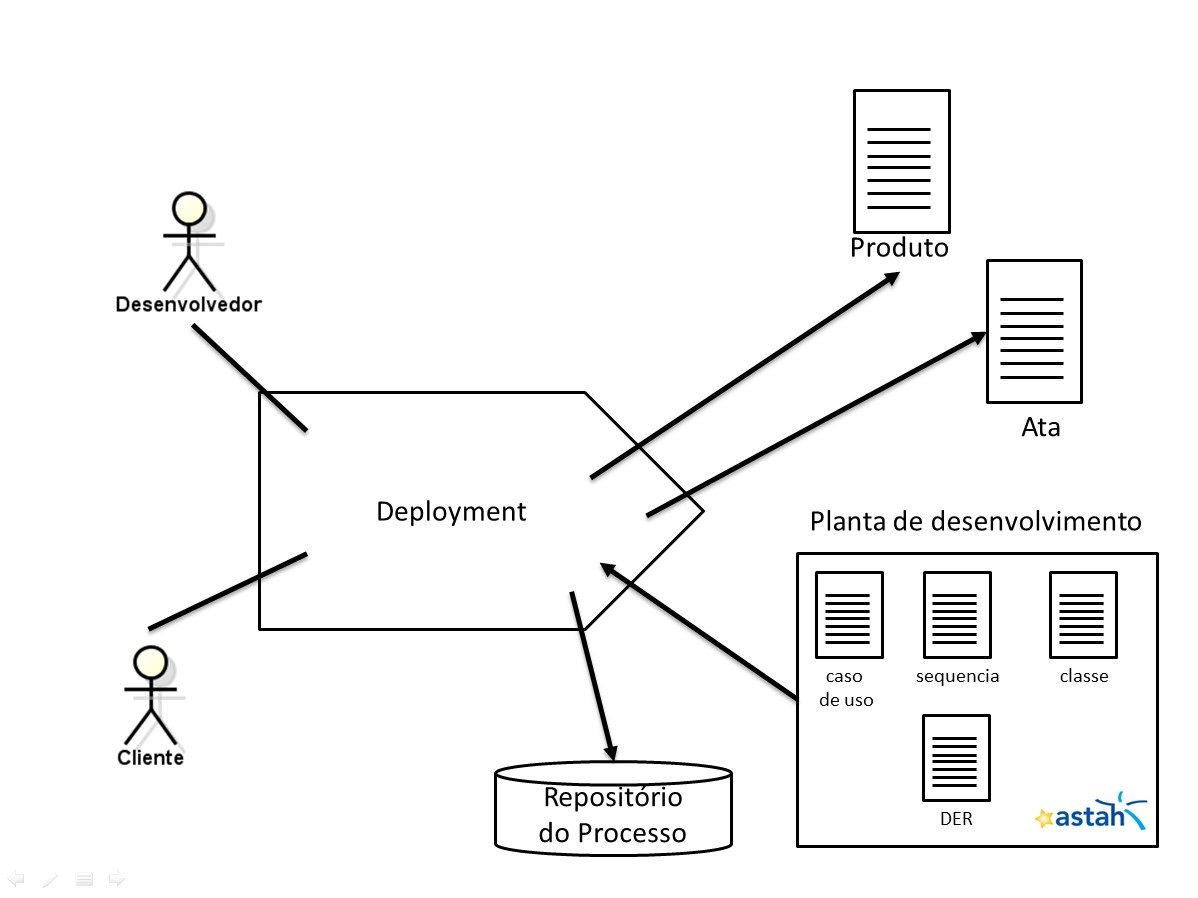
\includegraphics[scale=0.33]{img/entrega-software.jpg}
\legend{Fonte: Website do Scrum Solo}
\end{figure}

\section{Gestão}
Também de forma periódica, ocorrem reuniões de acompanhamento e gestão do projeto. Nesta etapa, são avaliados o progresso do projeto bem como eventuais mudanças de escopo, mudanças estas que podem alterar os artefatos elaborados até então. A Figura \ref{gestao} mostra como fica o relacionamento dos atores com os artefatos nesta etapa.

\begin{figure}[H]
\caption{\label{gestao} Gestão de projeto}
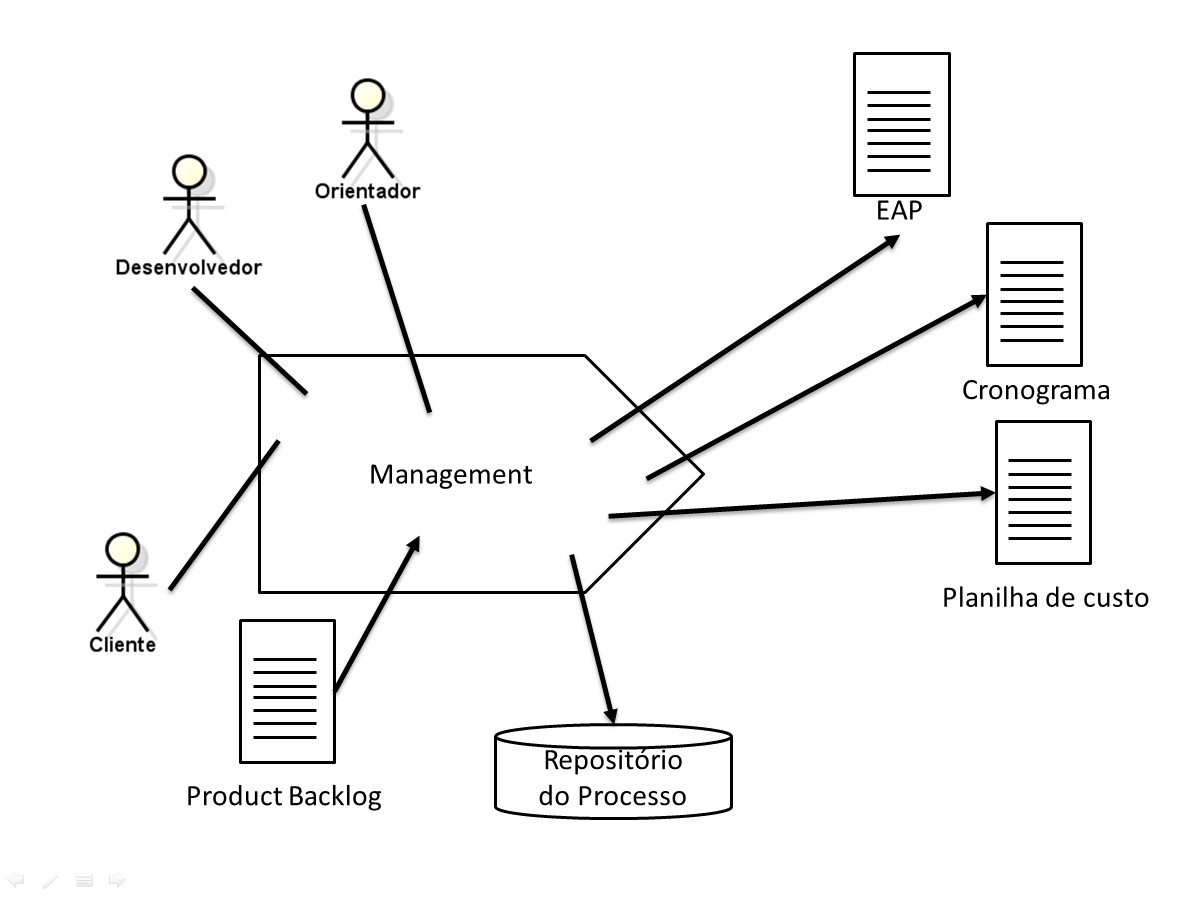
\includegraphics[scale=0.33]{img/gestao.jpg}
\legend{Fonte: Website do Scrum Solo}
\end{figure}

\section{Repositório de artefatos}
O Scrum Solo prevê a existência de um repositório na nuvem para todos os artefatos que compõem um projeto, neste projeto é usado o seguinte endereço Scrum-Repo\footnote{https://www.dropbox.com/sh/ku5z0fzbermoq49/AACzrYhZ4mBv89ZaJfMosRHKa?dl=0}.

\section{Scrum solo neste projeto}
O desenvolvimento deste projeto, através da adaptação deste framework, mostrou-se muito produtivo. A oferta de documentos de modelo para dar início ao projeto propriamente dito, é muito prático e eficiente. O projeto de exemplo também ajuda muito na hora de fazer a estruturação do projeto e de definir uma maneira de interagir com o orientador. Utilizamos os seguintes artefatos nesta implementação:

\begin{itemize}
    \item[a)] Documento de escopo;
    \item[b)] User stories;
    \item[c)] Product backlog;
    \item[d)] Sprint backlog;
    \item[e)] Retrospectiva de sprint;
    \item[f)] Calendário de reuniões com o orientador do projeto.
\end{itemize}

